%%%%%%%%%%%%%%%%%%%%%%%%%%%%%%%%%%%%%%%%%%%%%%%%%%%%%%%%%%%%%%%%%%%%%%%%%%%%%%%
\chapter{Background}\label{ch:background}
%%%%%%%%%%%%%%%%%%%%%%%%%%%%%%%%%%%%%%%%%%%%%%%%%%%%%%%%%%%%%%%%%%%%%%%%%%%%%%%

%%%%%%%%%%%%%%%%%%%%%%%%%%%%%%%%%%%%%%%%%%%%%%%%%%%%%%%%%%%%%%%%%%%%%%%%%%%%%%%
\section{Complex Algebraic Geometry}\label{sec:background-complex-algebraic-geometry}
%%%%%%%%%%%%%%%%%%%%%%%%%%%%%%%%%%%%%%%%%%%%%%%%%%%%%%%%%%%%%%%%%%%%%%%%%%%%%%%

This section serves as a brief introduction to the theory of complex algebraic
curves. Primary references are % TODO - griffiths and ueno references

%..............................................................................
\subsection{The Projective Line}
%..............................................................................

The primary motivation behind complex projective geometry is to make concrete
the way in which we analyze the behavior of functions, such as polynomials, at
infinity without having to resort to techniques separate from those used at
finite points. For example, in applications we may need to integrate a
differential along a path on an algebraic curve going to infinity. Knowing the
geometry of the curve at infinity makes such an operation computationally
feasible.

In fact, anyone with an elementary complex analysis background has seen an
example of projective geometry. The Riemann sphere is the complex plane $\CC$
with a ``point at infinity'' added. Let $z$ denote the coordinate in $\CC$
(i.e., the point $z=0$ represents the origin of the complex plane). In order to
discuss the point at infinity we introduce the coordinate $w = 1/z$. The
analysis of some function at $\infty$ is equivalent to rewriting the problem in
terms of the coordinate $w$ and examining its behavior in a neighborhood of
$w=0$. This explains why, for example, the exponential function
\[
  e^z = \sum_{n=0}^\infty z^n / n!,
\]
though entire in the complex plane, has an essential singularity on the Riemann
sphere since the exponential function in the coordinate $w$ centered at $w=0$ is
expressed by the series
\[
  \sum_{n=0}^\infty \frac{w^{-n}}{n!}.
\]

This point at infinity is not rigorously defined because it does not make sense
to {\it equate} $z=\infty$. The definition of the Riemann sphere is made
explicit by the following construction: consider the set $U = \CC^2 -
\{(0,0)\}$. Define the equivalence relation
\[
  (a_0, a_1) \sim (\lambda a_0, \lambda a_1), \quad \forall \lambda \in \CC -
  \{0\}.
\]
Thus two points $(a_0,a_1)$ and $(b_0,b_1)$ in $U$ are considered the same if
the ratios $a_0 : a_1$ and $b_0 : b_1$ are equal. The set of all points
$(b_0,b_1)$ equal to $(a_0,a_1)$ is called the {\it equivalence class} of
$(a_0,a_1)$ and the {\it complex projective line} $\PP{1}\CC$ is the set of all
such equivalence classes. That is,
\[
  \PP{1}\CC := \CC^2 / \sim.
\]
The equivalence class of $(a_0,a_1)$, called a ``point'' in $\PP{1}\CC$, is
written $(a_0 : a_1) \in \PP{1}\CC$. $\PP{1}\CC$ is precisely the Riemann
sphere. To see this, consider the two subsets
\begin{align*}
  U_0 &= \{ (a_0 : a_1) \in \PP{1}\CC \; | \; a_0 \neq 0 \}, \\
  U_1 &= \{ (a_0 : a_1) \in \PP{1}\CC \; | \; a_1 \neq 0 \}.
\end{align*}
For any $(a_0 : a_1) \in U_0$ we have, by the equivalence property,
\[
  (a_0 : a_1) = (1 : a_1/a_0) = (1 : a).
\]
Similarly, $(b_0 : b_1) = (b : 1)$ for every point in $U_1$. Every point in the
intersection $U_0 \cap U_1$ can be written in either of these two forms. Each of
these subspaces are isomorphic to $\CC$ since the maps
\begin{align*}
  \phi_0 : U_0 \to \CC,
  \quad
  \phi_0 \left( (a_0 : a_1) \right) = a_1 / a_0,
  & \quad \text{ and } \\
  \phi_1 : U_1 \to \CC,
  \quad
  \phi_1 \left( (a_0 : a_1) \right) = a_0 / a_1, &
\end{align*}
are continuous bijections with inverses
\begin{gather}
  \phi^{-1}_0(a) = (1 : a), \\
  \phi^{-1}_1(b) = (b : 1).
\end{gather}
Finally, note that $(0 : 1)$ is the only projective point in $U_1$ which is not
in $U_0$. Therefore, we identify $U_0$ with the complex plane (in the coordinate
$z$) and the point $P_\infty = (0 : 1)$ with the point at infinity and set
\begin{equation} \label{eqn: projective-line}
  \PP{1}\CC = U_0 \cup \{ (0 : 1) \} \cong \CC \cup P_\infty.
\end{equation}

Indeed $P_\infty$ is considered the point at infinity on the Riemann sphere for
if one considers the image of $(0 : 1)$ under $\phi_0$, though undefined since
$(0:1) \not \in U_0$, it maps to $z = 1 / 0$ ``='' $\infty$. Again, this does
not make sense without the complex projective space construction above but is
merely used to illustrate the point. The coordinate transformation from $z$ to
$w$ at the beginning of this section is equivalent to identifying $U_1$ with the
complex plane $\CC$ and $\{(1 : 0)\}$ with the point at infinity, instead.

%------------------------------------------------------------------------------
\subsection{The Projective Plane}
%------------------------------------------------------------------------------

The natural environment we use in the sequel is not the complex projective line
but the complex projective plane. In this section we construct the projective
plane and examine its geometric properties. The construction is similar to that
of the projective line.

Let $U = \CC^3 - \{(0,0,0)\}$. Following the strategy of the previous section,
consider the set of all ratios $(a_0 : a_1 : a_2)$, that is, the collection of
all equivalence classes under the equivalence relation $(a_0 : a_1 : a_2) \sim
(\lambda a_0 : \lambda a_1 : \lambda a_2), \forall \lambda \in \CC - \{0\}$. The
space of all such equivalence classes is called the two-dimensional complex
projective space or {\it the projective plane} and is denoted $\PP{2}\CC$.

Define the subsets $U_0,U_1,U_2$ by
\[
  U_j = \{ (a_0 : a_1 : a_2) \in \PP{2}\CC \; | \; a_j \neq 0 \},
\]
and note that all $(a_0 : a_1 : a_2) \in U_0$ satisfy $(a_0 : a_1 : a_2) = (1 :
a_1/a_0 : a_2/a_0)$. We define the bijective mapping
\begin{gather*}
  \phi_0 : U_0 \to \CC^2, \\
  \phi_0 \left( (a_0 : a_1 : a_2) \right) =
  \left( \frac{a_1}{a_0}, \frac{a_2}{a_0} \right), \\
  \phi_0^{-1} \left( (x,y) \right) = (1 : x : y).
\end{gather*}
The mappings $\phi_1$ and $\phi_2$ are similarly defined on $U_1$ and $U_2$,
respectively. Therefore, we can identify $U_0$ with the complex plane $\CC^2$.

Consider the space $U_0^c = \PP{2}\CC - U_0$. By definition, every point in
$U_0^c$ is of the form $(0 : a_1 : a_2)$. By definition, every point in $U_0^c$
determines a point on the complex projective line $\PP{1}\CC$. The converse is
true as well, resulting in the bijection
\[
  (0 : a_1 : a_2) \in \PP{2}\CC \; \leftrightarrow \; (a_1 : a_2) \in \PP{1}\CC.
\]
By identifying $U_0^c$ with $\PP{1}\CC$ we may write
\begin{equation} \label{eqn: proejctive-plane} \PP{2}\CC = U_0 \cup U_0^c \cong
  \CC^2 \cup \PP{1}\CC
\end{equation}
where $U_0^c \cong \PP{1}\CC$ is called the {\it line at infinity}, denoted
$l_\infty$, and $U_0 \cong \CC^2$ is called the {\it complex affine plane}. We
may also identify the complex affine plane with the sets $U_1$ or $U_2$ and the
line at infinity with their complements.

We saw a natural geometric interpretation of $\PP{1}\CC$ in the previous
section. Does such an interpretation exist for $\PP{2}\CC$? Consider a line in
the complex affine plane $\CC^2$ which can be written in the form
\[
  \alpha + \beta x + \gamma y = 0, \quad \text{where } (\beta,\gamma) \neq 0,
  \alpha, \beta, \gamma \in \CC.
\]
Using the inverse mapping $\phi_0^{-1}$ on $\CC^2$ we have
\[
  x = \frac{x_1}{x_0} \text{ and } y = \frac{x_2}{x_0},
\]
where $(x_0 : x_1 : x_2)$ are the coordinates of $\PP{2}\CC$, and we get the
line
\[
  \alpha x_0 + \beta x_1 + \gamma x_2 = 0.
\]
This equation, called the {\it homogenization} of the affine curve, makes sense
in all of $\PP{2}\CC$. Setting $x_0 = 1$ gives the original affine line. On the
other hand, setting $x_0 = 0$ gives the equation
\[
  \beta x_1 + \gamma x_2 = 0,
\]
which is the equation of the line in $l_\infty$. However, this implies $x_1 /
x_2 = - \gamma / \beta$. Hence the projective point $(0 : -\gamma : \beta)$
satisfies the equation
\[
  \alpha x_0 + \beta x_1 + \gamma x_2 = 0
\]
and is, in fact, the only projective point in $l_\infty$ on the line.

This means that the line ``intersects'' $l_\infty$ at the point $(0 : -\gamma :
\beta)$ and that this intersection point depends only on the slope of the affine
portion of the line. Hence, the line at infinity has the geometric meaning that
each point on it is the intersection point of an entire family of parallel lines
in $\CC^2$. This leads to a generalization of a theorem from classical planar
geometry: {\it any two, distinct lines in $\PP{2}\CC$ intersect at exactly one
  point}.

%------------------------------------------------------------------------------
\subsection{Projective Plane Curves} \label{sec: projective-plane-curves}
%------------------------------------------------------------------------------

The set of all points $(x_0, x_1, x_2)$ satisfying
\[
  \alpha x_0 + \beta x_1 + \gamma x_2 = 0
\]
is called a projective line and is a simple example of a projective algebraic
curve (of degree one). In this section we introduce various properties of
general projective curves.

An {\it complex plane algebraic curve} is the zero locus of the homogenization
of a polynomial $f \in \CC[x,y]$. That is, given a polynomial $f(x,y) =
\alpha_n(x) y^n + \alpha_{n-1}(x)y^{n-1} + \cdots + \alpha_0(x)$ its
homogenization is the polynomial $F \in \PP{2}\CC[x_0,x_1,x_2]$ where
\[
  F(x_0,x_1,x_2) = x_0^d f(x_1/x_0,x_2/x_0).
\]
where $d$ is the degree of $F$. The homogeneity of $F$ means that we can write
\[
  F(x_0,x_1,x_2) = \sum_{i+j+k=d} \alpha_{ijk} x_0^i x_1^j x_2^k.
\]

In terms of the projective polynomial $F$, its affine part can be written
$f(x,y) = F(1,x,y)$. As in the case of a projective line, $f$ can be thought of
as a projection of the polynomial $F$ onto $\CC^2$ and there is always a
one-to-one correspondence between an affine polynomial and its homogenization.
Therefore, a {\it complex plane algebraic curve} is the set
\[
  C = \left\{ (x_0 : x_1 : x_2) \in \PP{2}\CC : F(x_0,x_1,x_2) = 0 \right\}.
\]

Important to the study of projective curves, and specifically in the
computational work described here, are singular points.
\begin{definition} \label{def: singular-point} A point $a = (a_0 : a_1 : a_2)
  \in C$ is a {\bf singular point of $C$}, or a {\it multiple point of $C$}, if
  \[
    \left( \frac{\partial F}{\partial x_0},
      \frac{\partial F}{\partial x_1},
      \frac{\partial F}{\partial x_2} \right) (a) = (0,0,0).
  \]
\end{definition}
Consider the case when $a = (1 : 0 : 0)$ (corresponding to the point $(0,0)$ in
the affine plane $\CC^2$) is a singular point of $F$. The affine poirtion of the
curve is
\[
  f(x,y) = \sum_{i+j \geq 2}^d c_{ij} x^iy^j.
\]
Note that the constant term is zero since $(0, 0)$ is a point on the affine
curve and the linear term vanishes since $(0,0)$ is a singular point. We write
\[
  f(x,y) = f_m(x,y) + f_{m+1}(x,y) + \cdots + f_d(x,y), \quad m \geq 2,
\]
where each $f_n$ is the sum of all terms of $f$ of degree $n$; that is, terms of
the form $c_{ij}x^iy^j$ such that $i+j=n$. The smallest such $m$ with non-zero
term $f_m$ appearing in $f$ is called the {\it multiplicity} of the singular
point $(1 : 0 : 0)$. Singularities with multiplicity two are called {\it double
  points}, those with multiplicity three are called {\it triple points}, and so
on.

The homogeneous term $f_m$ can be factored into linear factors
\[
  f_m(x,y) = \prod_{j=1}^m (\alpha_j x - \beta_j y).
\]
We call the space $f_m(x,y) = 0$ the {\it tangent cone of the plane curve $C$}
at $a = (1 : 0 : 0)$ consistsing of a finite number of intersecting lines $L_j :
\alpha_j x - \beta_j y$.

When a generic affine point $a = (1 : c : d)$ is a singular point we write the
affine curve in the form
\[
  f(x,y) = \sum_{i+j \geq 2}^d \tilde{c}_{ij} (x-c)^i(y-d)^j
\]
which we can write as a sum of polynomials $g_n(x-c,y-d)$ homogenous in $x-c$
and $y-d$.

In the case when the singular point $a = (0 : 1 : b) \in l_\infty$ we repeat the
above process with the affine curve
\[
  g(u,v) = \frac{1}{x_1^d} F(x_0, x_1, x_2) = F(u,1,v), \quad u =
  \frac{x_0}{x_1}, v = \frac{x_2}{x_1},
\]
which is a projection of $F$ onto $U_1 \cong \CC$ instead of $U_0$. We write $g$
as a sum of terms of the form $g_{ij}u^i(v-b)^j$. Finally, in the case $a = (0 :
0 : 1) \in l_\infty$ we use the affine curve
\[
  h(w,z) = \frac{1}{x_2^d} F(x_0, x_1, x_2) = F(w,z,1), \quad w =
  \frac{x_0}{x_2}, z = \frac{x_1}{x_2},
\]
and write $h$ as a sum of terms of the form $h_{ij}w^iz^j$.

\begin{example} \label{ex: 2-cubic}
Consider the cubic curve
\[
  C: F(x_0,x_1,x_2) = x_0^4 x_2^3 + 2 x_0^3 x_1^3 x_2 - x_1^7
\]
In complex affine space $x_0 = 1$ this curve is
\[
  f(x,y) = F(1,x,y) = y^3 + 2 x^3 y - x^7.
\]
A plot of $f$ for $x,y$ real is shown in Figure \ref{fig: example-cubic}. For $a
= (a_0 : a_1 : a_2)$ we have
\begin{align} \label{eq: singular-conditions}
  \frac{\partial F}{\partial x_0}(a)
  &=
  4 a_{0}^{3} a_{2}^{3} + 6 a_{0}^{2} a_{1}^{3} a_{2}, \notag \\
  \frac{\partial F}{\partial x_1}(a)
  &=
  6 a_{0}^{3} a_{1}^{2} a_{2} - 7 a_{1}^{6}, \notag \\
  \frac{\partial F}{\partial x_2}(a)
  &=
  3 a_{0}^{4} a_{2}^{2} + 2 a_{0}^{3} a_{1}^{3}.
\end{align}

\begin{figure}
  \centering
  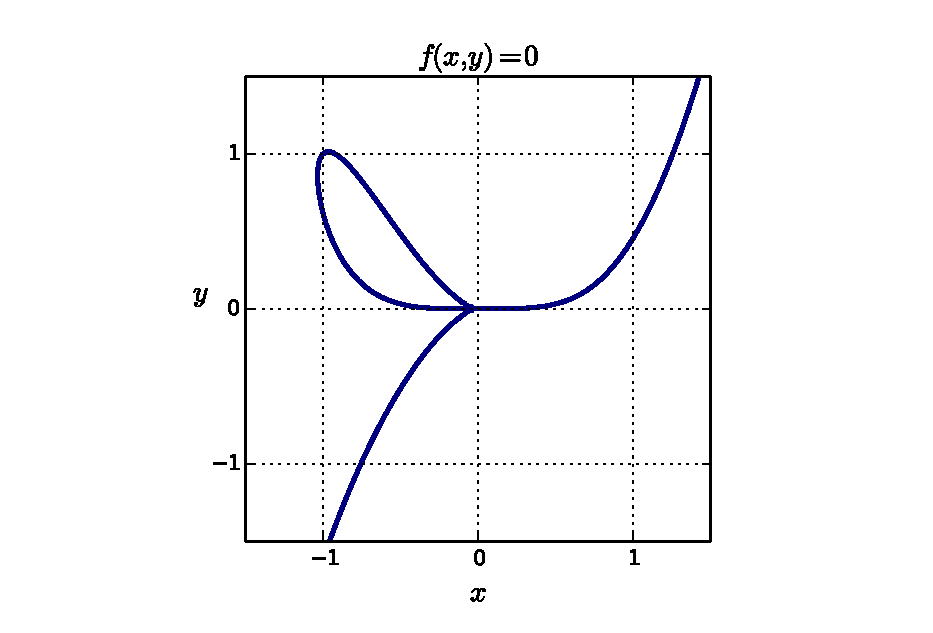
\includegraphics[width=0.9\textwidth]{images/singularities-example.eps}
  \caption{A real plot of the curve $C : f(x,y) = y^3 + 2 x^3 y - x^7$. The plot
    suggests that $(x_0 : x_1 : x_2) = (1 : 0 : 0)$, corresponding to $(x,y) =
    (0,0)$, is a singular point of $C$.}
  \label{fig: example-cubic}
\end{figure}

First, we find the finite singular points of $C$. Setting $a_0=1$ and solving
the above equations for $a_1$ and $a_2$ we see that $p = (1 : 0 : 0)$ is the
only finite singular point of $F$. Note that
\begin{gather*}
  f(x,y) = f_3(x,y) + f_4(x,y) + f_7(x,y), \\
  \\
  f_3(x,y) = y^3, \quad
  f_4(x,y) = 2 x^3 y, \quad
  f_7(x,y) = -x^7,
\end{gather*}
and that $f_3$, $f_4$, and $f_7$ are homogeneous of degrees 3, 4, and 7,
respectively. Therefore, $p$ is a singular point of multiplicity 3 with
\[
  f_3(x,y) = y^3 = 0,
\]
as the equation for the tangent cone at $p$. These properties are suggested by
Figure \ref{fig: example-cubic} where, near the point $p$, the real curve looks
like the intersection of three curves well approximated by the line $y = 0$ near
the point $x = 0$.

Setting $a_0 = 0$, the only expression in Equation \eqref{eq:
  singular-conditions} that does not reduce to zero is
\[
  \frac{\partial F}{\partial x_1}((0,a_1,a_2)) = - 7 a_{1}^{6} = 0,
\]
implying that the point $a = (0 : 0 : 1)$ is the only singular point at
infinity. The curve at infinity centered at $(0 : 0 : 1)$ is
\[
  h(w,z) = F(w,z,1) = w^{4} + 2 w^{3} z^{3} - z^{7}.
\]
The order of this singularity is four since this is the degree of the lowest
degree homogeneous term. The tangent cone at $a$ is $g_4(w,z) = w^4$.
\end{example}


%------------------------------------------------------------------------------
\subsection{Connection to Riemann Surfaces}
%------------------------------------------------------------------------------

There is a close relationship between the study of compact Riemann surfaces and
that of algebraic curves. Recall that a Riemann surface $X$ is a complex
manifold of complex dimension one endowed with an {\it atlas}: an open covering
$\{U_\alpha \}_{\alpha \in A}$ of $X$ together with a collection of
homeomorphisms $\{z_\alpha : U_\alpha \to \CC\}_{\alpha \in A}$, called {\it
  local parameters}, such that every pair of {\it transition functions}
\[
  f_{\beta,\alpha} := z_\beta \circ z_\alpha^{-1} : z_\alpha \left( U_\alpha
    \cap U_\beta \right) \to z_\beta \left( U_\alpha \cap U_\beta \right),
\]
is holomorphic. The pairs $(U_\alpha, z_\alpha)$ are called {\it coordinate
  charts}. In other words, a Riemann surface is a topological space such that
for all $P \in X$ there is a neighborhood of $P$ homeomorphic to an open subset
of the complex plane and one can analytically continue from any $P \in X$ to any
$Q \in X$ via transition functions.

The Riemann sphere $X = \CC^*$ is an example of a Riemann surface. Its atlas
consists of two coordinate charts $(U_1, z_1)$ and $(U_2, z_2)$ with
\begin{align*}
  U_1 = \CC, & \quad z_1 = z, \\
  U_2 = \left( \CC - \{0\} \right) \cup \{ \infty \}, & \quad z_2 = 1/z.
\end{align*}
This is a valid atlas since the transition functions
\begin{gather*}
  f_{1,2}, f_{2,1} : \left(\CC - \{0\}\right)
  \to \left(\CC - \{0\}\right) \\
  f_{1,2} = z_1 \circ z_2^{-1} = 1/z \\
  f_{2,1} = z_2 \circ z_1^{-1} = 1/z
\end{gather*}
are holomorphic on $U_1 \cap U_2 = \CC - \{0\}$.

These relationships between curves and Riemann surfaces are embodied by the
following two theorems % TODO Griffiths reference

\begin{theorem} \label{thm: normalization} {\bf (Normalization Theorem.)} For
  any irreducible algebraic curve $C \subset \PP{2}\CC$ there exists a compact
  Riemann surface $X$ and a holomorphic mapping
  \[
    \sigma : X \to \PP{2}\CC,
  \]
  such that $\sigma( X ) = C$ and $\sigma$ is injective on the inverse image of
  the set of smooth points of $C$.
\end{theorem}

A Riemann surface together with the mapping $\sigma$ is called the {\it
  normalization of $C$}. Loosely speaking, the normalization theorem states that
an algebraic curve is a Riemann surface except at the singular points.

Conversely, every compact Riemann surface can be represented by an algebraic
curve.
\begin{theorem} \label{thm: repr-theorem} Any compact Riemann surface $X$ can be
  obtained through the normalization of a certain plane algebraic curve $C$ with
  at most ordinary double points. That is, there exists a holomorphic mapping
  \[
    \sigma : X \to \PP{2}\CC
  \]
  such that $\sigma(X)$ is an algebraic curve possessing at most ordinary double
  points.
\end{theorem}
Many of the geometric algorithms presented in this document are designed to
avoid singular points. Except, for example, when we want to integrate a 1-form
along a path leading to a singular point in which case we ``unwrap'' the
singularity using Puiseux series. This is discussed in more detail in the
following section. However, because of this we use the terms ``curve'' and
``Riemann surface'' interchangably.

Additionally, the algorithms presented in this document primarily work with the
affine part $f(x,y)$ of the curve $F(x_0,x_1,x_2)$. If analysis on the line at
infinity is necessary, for example, when computing the singular points of a
curve, we consider an affine projection $g$ of $F$ onto $l_\infty$,
\[
  g(u,y) = u^d f(1/u,y) = 0.
\]

Thus, the surface considered here is the branched algebraic $y$-covering of the
complex $x$-Riemann sphere, the set of all $(x,y)$-solutions to the affine
polynomial equation
\[
    C = \{ (x,y) \in \CC \; | \; f(x,y) = \alpha_d(x)y^d +
    \alpha_{d-1}y^{d-1} + \cdots + \alpha_1(x)y + \alpha_0(x) = 0\},
\]
as $x$ varies along all of $\CC$. We treat $x$ and $y$ as the independent and
dependent variables of the equation, respectively.

A {\it point} $\alpha \in \CC$ is called a {\it regular point of $C$} if
\[
  f(\alpha,y) = 0
\]
has $d$ distinct $y$-roots $y_0,\ldots,y_{d-1}$. A point $\alpha \in \CC$ is
called a discriminant point if it is not regular. The point $\alpha = \infty$ is
a regular point of $C$ if
\[
  g(0,y)
\]
has $d$ disctinct roots.

A {\it place} $P$ is an element of $X$. For all but finitely many places, $P$ is
given by a pair $(\alpha,\beta)$ such that $f(\alpha,\beta) = 0$. However, some
places, particularly those where $\alpha$ is a discriminant point, instead needs
to be represented by a pair of series $(x(t),y(t))$ in some local coordinate
$t$. This will be discussed in more detail in the following section.


%%%%%%%%%%%%%%%%%%%%%%%%%%%%%%%%%%%%%%%%%%%%%%%%%%%%%%%%%%%%%%%%%%%%%%%%%%%%%%%
\section{Algebraic Curves}\label{sec:background-algebraic-curves}
%%%%%%%%%%%%%%%%%%%%%%%%%%%%%%%%%%%%%%%%%%%%%%%%%%%%%%%%%%%%%%%%%%%%%%%%%%%%%%%

%%%%%%%%%%%%%%%%%%%%%%%%%%%%%%%%%%%%%%%%%%%%%%%%%%%%%%%%%%%%%%%%%%%%%%%%%%%%%%%
\subsection{Puiseux Series}\label{subsec:background-puiseux-series}
%%%%%%%%%%%%%%%%%%%%%%%%%%%%%%%%%%%%%%%%%%%%%%%%%%%%%%%%%%%%%%%%%%%%%%%%%%%%%%%

Every analytic function $f = f(x)$ admits a local Taylor series representation
in a neighborhood about $x = \alpha$. If the function is meromorphic it still
admits a local series representation in the form of a Laurent series. An
extension of Taylor series are the Laurent series
\[
    f(x) = \sum_{n=N}^\infty c_n (x-\alpha)^n
\]
for some $N \in \ZZ \cup \{-\infty\}$ depending on $\alpha$. In both of these
situations the variable $x$ is a {\it local coordinate} of $f$ near the point
$\alpha$.

For algebraic curves, local coordinates are given in terms of Puiseux series,
which can be thought of as an extension of Laurent series.
\begin{definition} \label{def: puiseux} A {\bf Puiseux series} expansion of a
  curve $C : f(x,y) = 0$ at the point $x=\alpha$ is a collection of $j =
  1,\ldots,m \leq d = \text{deg}_y f$ series of the form
  \begin{align*}
    P_j(t) =
    \begin{cases}
      x_j(t) = \alpha + \lambda_j t^{e_j}, \\
      y_j(t) = \sum_{k=N}^\infty \beta_{jk} t^{n_{jk}},
    \end{cases}
  \end{align*}
  where $N \in \ZZ \cup \{-\infty\}$, $\alpha, \lambda_j, \beta_{jk} \in \CC$,
  and $e_j,n_{jk} \in \ZZ$. Each Puiseux series $P_j$ is a ``place'' on $C$.
\end{definition}
A place $P_j = P_j(t)$ satisfies
\[
    f\big(P_j(t)\big) := f\big(x_j(t), y_j(t)\big) = 0.
\]
When a Puiseux series $P_j(t)$ represents an expansion about a non-singular
$(\alpha, \beta_j)$ on the curve then $P(0) = (\alpha,\beta)$. This is not
necessarily the case about singular places. We list some additional important
facts and properties of Puiseux series.
\begin{itemize}
\item The integer $|e_j|$ is called the {\it branching number} or {\it
    ramification index} of the series expansion at that place: $|e_j| > 1$ when
  $x = \alpha$ is a branch point of the curve.
\item The number of Puiseux series $m$ at a branch point $x = \alpha$ is
  strictly less than $d = \text{deg}_y f$. However, $d = \sum_{j=1}^m |e_j|$.
\item The field of Puiseux series is a splitting field for $\CC[x,y] =
  \CC[x][y]$. That is, given any $f \in \CC[x,y]$ and Puiseux series expansions
  about any $x=\alpha$ we can write
  \[
    f(x,y) = \prod_{j=1}^m \prod_{k=1}^{e_j} \left( y - y_j\left(
             (e/\lambda_j)^{2 \pi ik / e_j}(x-\alpha) \right) \right),
  \]
  where the first product ranges over all Puiseux series $P_j$ at $x=\alpha$ and
  the second product ranges over all $y$-components $y_j(x_j)$ when solving for
  $t$ in terms of $x$. Note that a Puiseux series $P_j$ with ramification index
  $|e_j|>1$ splits into $|e_j|$ $y$-series in $x$.
\end{itemize}

\begin{example} \label{ex: 3-puiseux} Consider the curve
  \[
      C : f(x,y) = y^3 + 2x^3y - x^7 = 0.
  \]
  As seen in Example \ref{ex: 2-cubic}, the point $(x,y) = (0,0)$ is a singular
  point of $C$. The Puiseux series expansions lying above $x=0$ are all of the
  form
  \begin{align*}
    P_1(t) &=
             \begin{cases}
               x(t) = t, \\
               y(t) = \frac{t^{4}}{2} - \frac{t^{9}}{16} + \frac{3 t^{14}}{128}
               + \cdots,
             \end{cases} \\
    P_2(t) &=
             \begin{cases}
               x(t) = - \frac{t^{2}}{2}, \\
               y(t) = - \frac{t^{3}}{2} - \frac{t^{8}}{64} + \frac{3
                 t^{13}}{4096} + \cdots.
             \end{cases}
  \end{align*}
  We compute these expansions using {\tt abelfunctions}.

  % TODO - check the syntax below
  \begin{lstlisting}[language=Sage]
    sage: from abelfunctions import *
    sage: R.<x,y> = QQ[]   # construct the polynomial ring Q[x,y]
    sage: f = y**3 + 2*x**3*y - x**7
    sage: alpha = 0
    sage: P = puiseux( % TODO
    sage: print P[0]
    % TODO
    sage: print P[1]
    % TODO
  \end{lstlisting}
\end{example}

%%%%%%%%%%%%%%%%%%%%%%%%%%%%%%%%%%%%%%%%%%%%%%%%%%%%%%%%%%%%%%%%%%%%%%%%%%%%%%%
\subsection{Singularities}\label{subsec:background-singularities}
%%%%%%%%%%%%%%%%%%%%%%%%%%%%%%%%%%%%%%%%%%%%%%%%%%%%%%%%%%%%%%%%%%%%%%%%%%%%%%%

Recall from Definition \ref{def: singular-point} that a point $a$ on a
projective curve $C$ is a singular point if
\[
  \left( \frac{\partial F}{\partial x_0}, \frac{\partial F}{\partial x_1},
    \frac{\partial F}{\partial x_2} \right) (a) = (0,0,0).
\]
For singular points of the form $a = (1 : \alpha, \beta)$, this is equivalent to
\[
  \frac{\partial f}{\partial x} (\alpha,\beta) = 0, \quad \frac{\partial
    f}{\partial y} (\alpha,\beta) = 0,
\]
where $f$ is the affine portion of the curve. The singular points of a curve
need to be determined not only for the numerical analytic continuation and
integration methods discussed below, so we can appropriately desingularize the
curve $C$ and obtain a Riemann surface $X$, but they are also an essential
ingredient to computing a basis of holomorphic 1-forms on $X$.

A major role of Puiseux series is to provide a local coordinate chart at a
singular point. For singular points of the form $a = (1 : \alpha : \beta)$ the
Puiseux series expansion $P_j$ of $f = f(x,y)$ such that $P_j(0) = (\alpha,
\beta)$ is a coordinate chart centered at $(x,y) = (\alpha, \beta)$. $P_j$ tells
us how to approach and pass through $(x,y) = (\alpha, \beta)$ on the curve. With
this coordinate chart and those at other singular points of $C$ we can
desingularize the curve and thus create an appropriate atlas for the
corresponding Riemann surface $X$.

For the purposes of computing the genus of $X$ as well as the space of
holomorphic 1-forms $\Gamma(X,\Omega_X^1)$ on $X$ we need to compute the delta
invariant and the multiplicity of a singularity, respectively. The following
discussion assumes the singularity is finite. To analyze infinite singular
points we project the curve $C$ onto the line at infinity $l_\infty$ using the
method described in Section \ref{sec: projective-plane-curves}.

{\bf Branching number.} The branching number $R$ of a singular point
$(\alpha,\beta)$ is the sum of the branch numbers of the Puiseux series
expansions centered at $(x,y) = (\alpha,\beta)$. That is,
\[
  R \quad = \sum_{\substack{j \\ P_j(0)=(\alpha,\beta)}} |e_j|.
\]

{\bf Multiplicity.} As given in Section \ref{sec: projective-plane-curves}, the
multiplicity of a singular point is the degree of the lowest degree non-zero
homogeneous term appearing in the polynomial expression for the curve centered
at $(\alpha, \beta)$.

{\bf Delta invariant.} The delta invariant $\delta_P$ of a singularity $P$ is
the number of double points concentrated at the singularity. This is equal to
the number of quadratic factors $(\alpha_i x - \beta_i y)^2$ appearing in the
tangent cone at the singularity. Let $S$ be the set of all singular points,
finite and infinity, of $C$. Then the genus is given by
\begin{equation} \label{eqn: genus-formula}
  g = \frac{(d-1)(d-2)}{2} - \sum_{P \in S} \delta_P.
\end{equation}


%%%%%%%%%%%%%%%%%%%%%%%%%%%%%%%%%%%%%%%%%%%%%%%%%%%%%%%%%%%%%%%%%%%%%%%%%%%%%%%
\section{Riemann Surfaces}\label{sec:background-algebraic-curves}
%%%%%%%%%%%%%%%%%%%%%%%%%%%%%%%%%%%%%%%%%%%%%%%%%%%%%%%%%%%%%%%%%%%%%%%%%%%%%%%

%%%%%%%%%%%%%%%%%%%%%%%%%%%%%%%%%%%%%%%%%%%%%%%%%%%%%%%%%%%%%%%%%%%%%%%%%%%%%%%
\subsection{Places}\label{subsec:background-places}
%%%%%%%%%%%%%%%%%%%%%%%%%%%%%%%%%%%%%%%%%%%%%%%%%%%%%%%%%%%%%%%%%%%%%%%%%%%%%%%

%%%%%%%%%%%%%%%%%%%%%%%%%%%%%%%%%%%%%%%%%%%%%%%%%%%%%%%%%%%%%%%%%%%%%%%%%%%%%%%
\subsection{Divisors}\label{subsec:background-divisors}
%%%%%%%%%%%%%%%%%%%%%%%%%%%%%%%%%%%%%%%%%%%%%%%%%%%%%%%%%%%%%%%%%%%%%%%%%%%%%%%

%%%%%%%%%%%%%%%%%%%%%%%%%%%%%%%%%%%%%%%%%%%%%%%%%%%%%%%%%%%%%%%%%%%%%%%%%%%%%%%
\subsection{Homology}\label{subsec:background-homology}
%%%%%%%%%%%%%%%%%%%%%%%%%%%%%%%%%%%%%%%%%%%%%%%%%%%%%%%%%%%%%%%%%%%%%%%%%%%%%%%

%%%%%%%%%%%%%%%%%%%%%%%%%%%%%%%%%%%%%%%%%%%%%%%%%%%%%%%%%%%%%%%%%%%%%%%%%%%%%%%
\subsection{Holomorphic and Meromorphic
  Differentials}\label{subsec:background-holomorphic-and-meromorphic-differentials}
%%%%%%%%%%%%%%%%%%%%%%%%%%%%%%%%%%%%%%%%%%%%%%%%%%%%%%%%%%%%%%%%%%%%%%%%%%%%%%%

%%%%%%%%%%%%%%%%%%%%%%%%%%%%%%%%%%%%%%%%%%%%%%%%%%%%%%%%%%%%%%%%%%%%%%%%%%%%%%%
\subsection{Jacobian and Period
  Matrices}\label{subsec:background-jacobian-and-period-matrices}
%%%%%%%%%%%%%%%%%%%%%%%%%%%%%%%%%%%%%%%%%%%%%%%%%%%%%%%%%%%%%%%%%%%%%%%%%%%%%%%

%%%%%%%%%%%%%%%%%%%%%%%%%%%%%%%%%%%%%%%%%%%%%%%%%%%%%%%%%%%%%%%%%%%%%%%%%%%%%%%
\subsection{The Abel Map}\label{subsec:background-the-abel-map}
%%%%%%%%%%%%%%%%%%%%%%%%%%%%%%%%%%%%%%%%%%%%%%%%%%%%%%%%%%%%%%%%%%%%%%%%%%%%%%%

%%%%%%%%%%%%%%%%%%%%%%%%%%%%%%%%%%%%%%%%%%%%%%%%%%%%%%%%%%%%%%%%%%%%%%%%%%%%%%%
\subsection{The Riemann Constant
  Vector}\label{subsec:background-the-riemann-constant-vector}
%%%%%%%%%%%%%%%%%%%%%%%%%%%%%%%%%%%%%%%%%%%%%%%%%%%%%%%%%%%%%%%%%%%%%%%%%%%%%%%

%%%%%%%%%%%%%%%%%%%%%%%%%%%%%%%%%%%%%%%%%%%%%%%%%%%%%%%%%%%%%%%%%%%%%%%%%%%%%%%
\section{The Riemann Theta
  Function}\label{sec:background-riemann-theta-function}
%%%%%%%%%%%%%%%%%%%%%%%%%%%%%%%%%%%%%%%%%%%%%%%%%%%%%%%%%%%%%%%%%%%%%%%%%%%%%%%